\chapter{Application of the Thermodynamic Extremal Principle}\label{ch:tep_application}

In the following the generalized extremal principle is applied on the current model of particles and nodes, see \autoref{subsubsec:extremal-priciple-generalized} for details on the approach.
As before, an index of the currently regarded particle or node is neglected where appropriate for brevity.
The indices $\ldots_{\Upper}$ and $\ldots_{\Lower}$ are used to denote the upper resp.~lower neighbor of a node.
${\Nodes}$ is the set of all nodes present in the system and ${\Particles}$ the set of all particles, respectively.

\section{Choice of Variables}\label{sec:variables}

First, the internal state variables $\Vect\InternalStateVariable$, the internal state velocities $\Vect\InternalStateVelocity$ and the fluxes $\Vect\Flux$ must be chosen.
The feasibility of the approach heavily depends on this choice.

The choice of the fluxes is straightforward with the diffusional fluxes.
One has two diffusional fluxes from each node $\Flux_{\Upper}$ and $\Flux_{\Lower}$ to the upper respectively the lower neighbor, however the flux of the upper node to the lower and the flux from the lower to the upper are always equal due to constancy of mass.
So in the following only $\Flux_{\Upper}$ shall be regarded and $\Flux_{\Lower}$ is substituted by $-\Flux_{\Upper}$ where necessary.

The internal state variables are the polar coordinates of the nodes $\left[ \Radius, \Angle \right]$ with pole in their particle's center, since they determine the thermodynamic forces and the main aim of the simulation is to follow the time evolution of the particles and nodes.
The coordinates of the particles $\left[ \X_{\Particle}, \Y_{\Particle} \right]$ are not used as internal state variables, since they are unambiguously defined, if the coordinates of all nodes relative to their particle are known and also which nodes are in contact to each other.
Moreover, the velocities of particle coordinates $\dot\X_{\Particle}$ and $\dot\Y_{\Particle}$ are auxiliary variables (included in $\Vect\AuxiliaryVariable$) to ease formulation of the geometric constraints.

For numerical and equation formulation reasons, the internal state velocities $\dot\Radius$ and $\dot\Angle$ are replaced by the velocities of node shift along normal and tangential surface vectors $\dot\Shift_{\Normal}$ and $\dot\Shift_{\Tangential}$.
As they are determined, translation into new coordinates is directly possible using the relations obtained in the following sections.

The external state variables (such as temperature $\Temperature$ and pressure $\Pressure$) are not considered in the following, since they are assumed constant.

\chapter{Equation System}\label{ch:equation-system}


\section{Components of the Lagrangian Gradient}\label{sec:components-of-the-lagrangian-gradient}

The following table displays all components of the Lagrangian gradient to be solved for the application of the \gls{TEP}.
Node symbols $n$ or contact symbols $c$ in parentheses behind another symbol mean, that this symbol is local to the node or contact, thus there exist one distinct value for each node or contact.
$n_\Upper$ denotes the upper neighbor of the currently regarded node, as well as $n_\Lower$ the lower.
The equations are all formulated in terms of fluxes from one node to the upper neighbor $\Flux_{\Upper}$, since $\Flux_\Lower(n) = -\Flux_\Upper(n_\Lower)$ must be always fulfilled.
This saves one unknown per node.

\begin{longtblr}[
    label=none,
    entry=none,
    note{*}={Only if the node is in parent position.}
]{
    colspec={lX[c]},
    measure=vbox
}
    \toprule
    \SetCell[c=2]{l} for each non-contact node $n$ \\
    \midrule
    $\LagrangeFunction_{\Step\Shift_\Normal(n)}$ &
    \begin{equation*}
        0
        = \frac{\partial\GibbsEnergy}{\partial\Shift_\Normal(n)} \left( 1 + \LagrangeParameter_1 \right)
        + \frac{\partial\Volume(n)}{\partial\Shift_\Normal(n)} \LagrangeParameter_{\Volume}(n)
    \end{equation*} \\

    $\LagrangeFunction_{\Flux_\Upper(n)}$ &
    \begin{equation*}
        0
        = \frac{2 \GasConstant \Temperature}{\MolarVolume \VacancyConcentration^\Standard} \frac{\SurfaceDistance_\Upper(n) \Flux_\Upper(n)}{\DiffusionCoefficient_\Upper(n)} \LagrangeParameter_1
        - \LagrangeParameter_\Volume(n)
        + \LagrangeParameter_\Volume(n_\Upper)
    \end{equation*} \\

    $\LagrangeFunction_{\LagrangeParameter_\Volume(n)}$ &
    \begin{equation*}
        0
        = \frac{\partial\Volume(n)}{\partial\Shift_\Normal} \Step\Shift_{\Normal}(n)
        - \Flux_{\Upper}(n)
        + \Flux_{\Upper}(n_\Lower)
    \end{equation*} \\

    \midrule
    \SetCell[c=2]{l} for each contact node $n$ as part of contact $c$ \\
    \midrule
    $\LagrangeFunction_{\Step\Shift_\Normal(n)}$ &
    \begin{equation*}
        0
        = \frac{\partial\GibbsEnergy}{\partial\Shift_\Normal(n)} \left( 1 + \LagrangeParameter_1 \right)
        + \frac{\partial\Volume(n)}{\partial\Shift_\Normal(n)} \LagrangeParameter_{\Volume}(n)
        - \frac{\partial \Radius_\Contact(c)}{\partial\Shift_\Normal(n)} \LagrangeParameter_{\Radius_\Contact}(n)
        - \frac{\partial \Angle_\Contact(c)}{\partial\Shift_\Normal(n)} \LagrangeParameter_{\Angle_\Contact}(n)
    \end{equation*} \\

    $\LagrangeFunction_{\Step\Shift_\Tangential(n)}$ &
    \begin{equation*}
        0
        = \frac{\partial\GibbsEnergy}{\partial\Shift_\Tangential(n)} \left( 1 + \LagrangeParameter_1 \right)
        + \frac{\partial\Volume(n)}{\partial\Shift_\Tangential(n)} \LagrangeParameter_{\Volume}(n)
        - \frac{\partial \Radius_\Contact(c)}{\partial\Shift_\Tangential(n)} \LagrangeParameter_{\Radius_\Contact}(n)
        - \frac{\partial \Angle_\Contact(c)}{\partial\Shift_\Tangential(n)} \LagrangeParameter_{\Angle_\Contact}(n)
    \end{equation*} \\

    $\LagrangeFunction_{\Flux_\Upper(n)}$ & same as above \\

    $\LagrangeFunction_{\LagrangeParameter_\Volume(n)}$ &
    \begin{equation*}
        0
        = \frac{\partial\Volume(n)}{\partial\Shift_\Normal} \Step\Shift_{\Normal}(n)
        + \frac{\partial\Volume(n)}{\partial\Shift_\Tangential} \Step\Shift_{\Tangential}(n)
        - \Flux_{\Upper}(n)
        + \Flux_{\Upper}(n_\Lower)
    \end{equation*} \\

    $\LagrangeFunction_{\LagrangeParameter_{\Radius_\Contact}(n)}$\TblrNote{*} &
    \begin{multline*}
        0
        = \Step\Radius_{\Contact}(c)
        - \frac{\partial \Radius_\Contact(c)}{\partial\Shift_\Normal(n)} \left( \Step\Shift_{\Normal}^{|\Parent}(n) + \Step\Shift_{\Normal}^{|\Child}(n) \right)
        - \frac{\partial \Radius_\Contact(c)}{\partial\Shift_\Tangential(n)} \left( \Step\Shift_{\Tangential}^{|\Parent}(n) + \Step\Shift_{\Tangential}^{|\Child}(n) \right) \\
        - 2 \frac{\partial \Radius_\Contact(c)}{\partial\Shift_\RotationAngle(n)} \Radius^{|\Child}(n) \sin \frac{\Step\RotationAngle_\Child(c)}{2}
    \end{multline*} \\

    $\LagrangeFunction_{\LagrangeParameter_{\Angle_\Contact}(n)}$\TblrNote{*} &
    \begin{multline*}
        0
        = \Step\Angle_{\Contact}(c)
        - \frac{\partial \Angle_\Contact(c)}{\partial\Shift_\Normal(n)} \left( \Step\Shift_{\Normal}^{|\Parent}(n) + \Step\Shift_{\Normal}^{|\Child}(n) \right)
        - \frac{\partial \Angle_\Contact(c)}{\partial\Shift_\Tangential(n)} \left( \Step\Shift_{\Tangential}^{|\Parent}(n) + \Step\Shift_{\Tangential}^{|\Child}(n) \right) \\
        - 2 \frac{\partial \Angle_\Contact(c)}{\partial\Shift_\RotationAngle(n)} \Radius^{|\Child}(n) \sin \frac{\Step\RotationAngle_\Child(c)}{2}
    \end{multline*} \\

    \midrule
    \SetCell[c=2]{l} for each contact $c$ with the therein involved nodes of the parent $\Nodes^{|\Parent}(c)$ \\
    \midrule
    $\LagrangeFunction_{\Step\Radius_\Contact(c)}$ &
    \begin{equation*}
        0
        = \sum^{\Nodes^{|\Parent}(c)}_n \LagrangeParameter_{\Radius_\Contact}(n)
    \end{equation*} \\

    $\LagrangeFunction_{\Step\Angle_\Contact(c)}$ &
    \begin{equation*}
        0
        = \sum^{\Nodes^{|\Parent}(c)}_n \LagrangeParameter_{\Angle_\Contact}(n)
    \end{equation*} \\

    $\LagrangeFunction_{\Step\RotationAngle_\Child(c)}$ &
    \begin{multline*}
        0
        = \sum^{\Nodes^{|\Parent}(c)}_n \Biggl[
            - \Radius^{|\Child}(n) \sin \left( \Step\RotationAngle_\Child(c) + \Angle^{|\Child}(n) - \Angle_\Contact^{|\Child}(c) \right) \LagrangeParameter_{\Radius_\Contact}(n) \\
            + \frac{\Radius^{|\Child}(n)}{\Radius_\Contact(c)} \cos \left( \Step\RotationAngle_\Child(c) + \Angle^{|\Child}(n) - \Angle_\Contact^{|\Child}(c)  \right) \LagrangeParameter_{\Angle_\Contact}(n)
            \Biggr]
    \end{multline*} \\

    \midrule
    \SetCell[c=2]{l} just once for the set of all nodes $\Nodes$ \\
    \midrule
    $\LagrangeFunction_{\LagrangeParameter_1}$ &
    \begin{equation*}
        0
        = \sum^\Nodes_n \left[
            \frac{\partial\GibbsEnergy}{\partial\Shift_\Normal(n)} \Step\Shift_\Normal(n)
            + \frac{\partial\GibbsEnergy}{\partial\Shift_\Tangential(n)} \Step\Shift_\Tangential(n)
            - \frac{\SurfaceDistance_\Upper(n) \Flux_\Upper(n)^2 + \SurfaceDistance_\Lower(n) \Flux_\Upper(n_\Lower)^2}{2\GasConstant\Temperature\MolarVolume\VacancyConcentration^\Standard}
            \right]
    \end{equation*} \\
    \bottomrule
\end{longtblr}


\section{Components of the Lagrangian Gradient's Jacobian}\label{sec:components-of-the-lagrangian-gradients-jacobian}
\section{Evolution of Particle Surfaces by Node Shifting}\label{sec:surface-evolution}

\begin{figure}
    \begin{subfigure}{\linewidth}
        \centering
        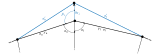
\includegraphics{img/model_development/node_shift_normal}
        \caption{Normal Direction}
        \label{fig:model_development/surface_normal}
    \end{subfigure}
    \begin{subfigure}{\linewidth}
        \centering
        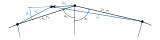
\includegraphics{img/model_development/node_shift_tangential}
        \caption{Tangential Direction}
        \label{fig:model_development/surface_tangential}
    \end{subfigure}
    \caption{Shifting of Surface Nodes}
    \label{fig:surface-node-shifting}
\end{figure}

\begin{figure}
    \begin{subfigure}{0.5\linewidth}
        \centering
        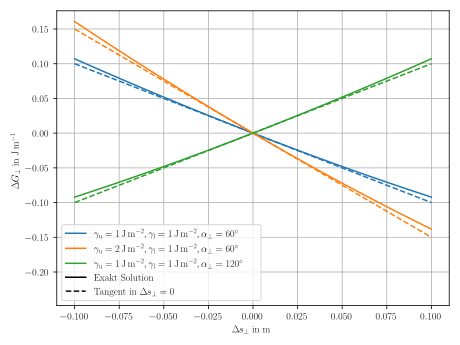
\includegraphics[scale=0.5]{img/model_development/plot_normal_potential}
        \caption{Normal Direction}
        \label{fig:model_development/plot_normal_potential}
    \end{subfigure}%
    \begin{subfigure}{0.5\linewidth}
        \centering
        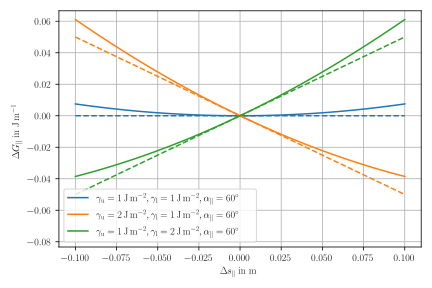
\includegraphics[scale=0.5]{img/model_development/plot_tangential_potential}
        \caption{Tangential Direction}
        \label{fig:model_development/plot_tangential_potential}
    \end{subfigure}
    \caption{Change in Gibbs Energy Due to Node Shifting (tangents dashed)}
    \label{fig:surface-node-potentials}
\end{figure}

In the following, the Gibbs energy and volume gradients when shifting nodes will be derived as needed in the formulation of dissipation $\Dissipation$ and dissipation function $\DissipationFunction$ given above.

\subsection{Normal Shifting}

The main mode of node shifting on free surfaces and grain boundaries is along the interface normal vector.
\autoref{fig:model_development/surface_normal} shows the principal geometry of a surface node and it's normal mode of shifting.

If a node is displaced in space, a change in Gibbs energy occurs due to the change in surface respectively interface area.
The amount of energy bound in a surface or interface is described by the interface energy $\InterfaceEnergy$.
Since a 2D problem is regarded, the length of the surface line $\SurfaceDistance$ is a measure of present surface area.
The change of Gibbs energy due to normal node shifting is described by \autoref{eq:gibbs-diff-surface-normal} with the prime values as measures after shifting.
\begin{equation}
    \Step\GibbsEnergy_{\Normal} = \left( \SurfaceDistance_{\Upper}' - \SurfaceDistance_{\Upper} \right) \InterfaceEnergy_{\Upper} +  \left(\SurfaceDistance_{\Lower}' - \SurfaceDistance_{\Lower} \right) \InterfaceEnergy_{\Lower}
    \label{eq:gibbs-diff-surface-normal}
\end{equation}

The normal vector points under an angle of $\SurfaceVectorAngle_\Normal$ acc.~to~\autoref{eq:delta-surface-normal} to both surface lines.
\begin{equation}
    \SurfaceVectorAngle_{\Normal} = \PI - \frac{1}{2} \left(\SurfaceRadiusAngle_{\Upper} + \SurfaceRadiusAngle_{\Lower} \right)
    \label{eq:delta-surface-normal}
\end{equation}

With a certain normal shift ${\Step\Shift}_\Normal$, the surface lengths after shifting are calculated by \autoref{eq:surface-distance-shifted-normal}.
\begin{subequations}
    \begin{align}
        \SurfaceDistance_{\Upper}' & = \sqrt{\SurfaceDistance_{\Upper}^2 + \Step\Shift_{\Normal}^2 - 2 \SurfaceDistance_{\Upper} \Step\Shift_{\Normal} \cos \SurfaceVectorAngle_{\Normal}} \label{eq:surface-distance-shifted-normal-upper}         \\
        \SurfaceDistance_{\Lower}' & = \sqrt{{\SurfaceDistance}_{\Lower}^2 + {\Step\Shift}_{\Normal}^2 - 2 {\SurfaceDistance}_{\Lower} {\Step\Shift}_{\Normal} \cos \SurfaceVectorAngle_{\Normal}} \label{eq:surface-distance-shifted-normal-lower}
    \end{align}
    \label{eq:surface-distance-shifted-normal}
\end{subequations}

\autoref{fig:model_development/plot_normal_potential} shows the change in Gibbs energy due to normal shifting with use of \autoref{eq:gibbs-diff-surface-normal} to \autoref{eq:surface-distance-shifted-normal} with different values of $\SurfaceVectorAngle_{\Normal}$ and $\InterfaceEnergy$, alongside the linear approximation around ${\Step\Shift}_{\Normal} = 0$.
Note, that the slope is dependent on the sum of ${\InterfaceEnergy}_{\Upper}$ and ${\InterfaceEnergy}_{\Lower}$ and the sign is only dependent on $\SurfaceVectorAngle_{\Normal}$.
$\SurfaceVectorAngle_{\Normal} > \qty{90}{\degree}$ means a convex surface, thus energy gain when inward shifting (negative ${\Step\Shift}_{\Normal}$).
$\SurfaceVectorAngle_{\Normal} < \qty{90}{\degree}$ means a concave surface, thus energy gain when outward shifting (positive ${\Step\Shift}_{\Normal}$).
$\SurfaceVectorAngle_{\Normal} = \qty{90}{\degree}$ means an even surface, thus energy loss in both shifting directions.

The partial derivative of Gibbs energy is obtained as the limit of $\Step\GibbsEnergy_{\Normal}$ when ${\Step\Shift}_{\Normal} \rightarrow 0$ as in \autoref{eq:gibbs-partial-surface-normal}.
\begin{equation}
    \frac{\partial \GibbsEnergy}{\partial {\Shift}_{\Normal}} = \lim_{\Step\Shift_{\Normal} \rightarrow 0} \frac{\Step\GibbsEnergy_{\Normal}}{\Step\Shift_{\Normal}} = -\left({\InterfaceEnergy}_{\Upper} + {\InterfaceEnergy}_{\Lower}\right) \cos \SurfaceVectorAngle_{\Normal}
    \label{eq:gibbs-partial-surface-normal}
\end{equation}

The volume derivative is obtained by calculating the area of the triangles formed by $\SurfaceDistance$, $\SurfaceDistance'$ and $\Step\Shift_{\Normal}$ on the upper and lower side.
\begin{subequations}
    \begin{align}
        \Step\Volume_{\Normal\Upper} &= \frac12 \SurfaceDistance_{\Upper} \Step\Shift_{\Normal} \sin \SurfaceVectorAngle_{\Normal} \\
        \Step\Volume_{\Normal\Lower} &= \frac12 \SurfaceDistance_{\Lower} \Step\Shift_{\Normal} \sin \SurfaceVectorAngle_{\Normal}
    \end{align}
    \label{eq:volume-diff-surface-normal}
\end{subequations}

The partial derivative of volume is obtained as the limit of $\Step\Volume_{\Normal\Upper} + \Step\Volume_{\Normal\Lower}$ when ${\Step\Shift}_{\Normal} \rightarrow 0$ as in \autoref{eq:volume-partial-surface-normal}.
\begin{equation}
    \frac{\partial \Volume}{\partial {\Shift}_{\Normal}} = \lim_{\Step\Shift_{\Normal} \rightarrow 0} \frac{\Step\Volume_{\Normal\Upper} + \Step\Volume_{\Normal\Lower}}{\Step\Shift_{\Normal}} = \frac{1}{2} \left( \SurfaceDistance_{\Upper} + \SurfaceDistance_{\Lower} \right) \sin \SurfaceVectorAngle_{\Normal}
    \label{eq:volume-partial-surface-normal}
\end{equation}

\subsection{Tangential Shifting}

Regarding the tangential shifting, the direction vector is under an angle of $\SurfaceVectorAngle_{\Tangential}$ acc.~to.~\autoref{eq:delta-surface-tangential} to the upper surface line.
\begin{equation}
    \SurfaceVectorAngle_{\Tangential} = \SurfaceVectorAngle_{\Normal} - \frac{\PI}{2}
    \label{eq:delta-surface-tangential}
\end{equation}

The change in Gibbs energy is calculated similarly as in the normal case according to \autoref{eq:gibbs-diff-surface-tangential}, but the shifted surface lengths are calculated as in \autoref{eq:surface-distance-shifted-tangential} in dependence on the tangential shift ${\Step\Shift}_{\Tangential}$.
Note especially the signs in front of the cosine terms.
\begin{equation}
    \Step\GibbsEnergy_{\Tangential} = \left( \SurfaceDistance_{\Upper}' - \SurfaceDistance_{\Upper} \right) \InterfaceEnergy_{\Upper} +  \left(\SurfaceDistance_{\Lower}' - \SurfaceDistance_{\Lower} \right) \InterfaceEnergy_{\Lower}
    \label{eq:gibbs-diff-surface-tangential}
\end{equation}
\begin{subequations}
    \begin{align}
        \SurfaceDistance_{\Upper}' & = \sqrt{{\SurfaceDistance}_{\Upper}^2 + {\Step\Shift}_{\Tangential}^2 - 2 {\SurfaceDistance}_{\Upper} {\Step\Shift}_{\Tangential} \cos \SurfaceVectorAngle_{\Tangential}} \label{eq:surface-distance-shifted-tangential-upper} \\
        \SurfaceDistance_{\Lower}' & = \sqrt{{\SurfaceDistance}_{\Lower}^2 + {\Step\Shift}_{\Tangential}^2 + 2 {\SurfaceDistance}_{\Lower} {\Step\Shift}_{\Tangential} \cos \SurfaceVectorAngle_{\Tangential}} \label{eq:surface-distance-shifted-tangential-lower}
    \end{align}
    \label{eq:surface-distance-shifted-tangential}
\end{subequations}

\autoref{fig:model_development/plot_tangential_potential} shows the change in Gibbs energy due to tangential shifting with different values of $\InterfaceEnergy$.
The slope and monotonicity of these curves is here dependent on the \emph{difference} of ${\InterfaceEnergy}_{\Upper}$ and ${\InterfaceEnergy}_{\Lower}$.
The convexity or concavity of the surface is here only of minor importance.
Whether the interface with higher $\InterfaceEnergy$ is located on the upper or lower side determines the monotonicity of the curves.
In the special case when ${\InterfaceEnergy}_{\Upper} = {\InterfaceEnergy}_{\Lower}$, the curve has a minimum in ${\Step\Shift}_{\Tangential} = 0$, meaning that any shift will produce an energy loss.
This is the case on all nodes except neck nodes.

Again, the partial derivative of Gibbs energy is found by the limit when ${\Step\Shift}_{\Tangential} \rightarrow 0$.
\begin{equation}
    \frac{\partial \GibbsEnergy}{\partial {\Shift}_{\Tangential}} = \lim_{\Step\Shift_{\Tangential} \rightarrow 0} \frac{\Step\GibbsEnergy_{\Tangential}}{\Step\Shift_{\Tangential}} = -\left({\InterfaceEnergy}_{\Upper} - {\InterfaceEnergy}_{\Lower}\right) \cos \SurfaceVectorAngle_{\Tangential}
    \label{eq:gibbs-partial-surface-tangential}
\end{equation}

The partial derivative of volume is found similarly as in the normal case, but the contribution of the lower side must be here counted negatively, as can be seen from \autoref{fig:model_development/surface_tangential}.
\begin{equation}
    \frac{\partial \Volume}{\partial {\Shift}_{\Tangential}} = \lim_{\Step\Shift_{\Tangential} \rightarrow 0} \frac{\Step\Volume_{\Tangential\Upper} - \Step\Volume_{\Tangential\Lower}}{\Step\Shift_{\Tangential}} = \frac{1}{2} \left( \SurfaceDistance_{\Upper} - \SurfaceDistance_{\Lower} \right) \sin \SurfaceVectorAngle_{\Tangential}
    \label{eq:volume-partial-surface-tangential}
\end{equation}

\subsection{Special Treatment of Neck Nodes}

\begin{figure}
    \begin{subfigure}{\linewidth}
        \centering
        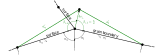
\includegraphics{img/model_development/node_shift_normal_neck}
        \caption{Normal Direction}
        \label{fig:model_development/node_shift_normal_neck}
    \end{subfigure}
    \begin{subfigure}{\linewidth}
        \centering
        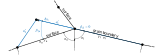
\includegraphics{img/model_development/node_shift_tangential_neck}
        \caption{Tangential Direction}
        \label{fig:model_development/node_shift_tangential_neck}
    \end{subfigure}
    \caption{Shifting of Neck Nodes}
    \label{fig:surface-node-shifting-neck}
\end{figure}

The neck nodes (triple points between two surfaces and one grain boundary) are a special case.
For numerical reasons, their shifting is not taken normal and tangential to the surface line, but only to the grain boundary, as this is in consistence with their primary evolution during sintering.
The case, where the grain boundary is located below the currently regarded node, is shown in \autoref{fig:surface-node-shifting-neck}.
Here, one must distinguish between the shift vector angles $\SurfaceVectorAngle$ to the upper and the lower surface line.
For the shown case the angles are as in \autoref{eq:shift-neck-angles}, if the grain boundary is, however, located above the node, than the values of the upper and lower angles have to be switched.
\begin{align}
    \SurfaceVectorAngle_{\Normal\Upper} = \frac32 \PI - \SurfaceRadiusAngle_{\Upper} - \SurfaceRadiusAngle_{\Lower} \qquad &\text{and} \qquad \SurfaceVectorAngle_{\Normal\Lower} = \frac\PI2 \\
    \SurfaceVectorAngle_{\Tangential\Upper} = \PI - \SurfaceRadiusAngle_{\Upper} - \SurfaceRadiusAngle_{\Lower} \qquad &\text{and} \qquad \SurfaceVectorAngle_{\Tangential\Lower} = 0
    \label{eq:shift-neck-angles}
\end{align}

The respective partial derivatives are slightly modified with the distinct angles as below.
\begin{align}
    \frac{\partial \GibbsEnergy}{\partial {\Shift}_{\Normal}} &= -\left( {\InterfaceEnergy}_{\Upper} \cos \SurfaceVectorAngle_{\Normal\Upper} - {\InterfaceEnergy}_{\Lower} \cos \SurfaceVectorAngle_{\Normal\Lower} \right)
    \label{eq:gibbs-partial-neck-normal} \\
    \frac{\partial \Volume}{\partial {\Shift}_{\Normal}} &= \frac{1}{2} \left( \SurfaceDistance_{\Upper} \sin \SurfaceVectorAngle_{\Normal\Upper} + \SurfaceDistance_{\Lower} \sin \SurfaceVectorAngle_{\Normal\Lower}\right)
    \label{eq:volume-partial-neck-normal} \\
    \frac{\partial \GibbsEnergy}{\partial {\Shift}_{\Tangential}} &= -\left( {\InterfaceEnergy}_{\Upper} \cos \SurfaceVectorAngle_{\Tangential\Upper} - {\InterfaceEnergy}_{\Lower} \cos \SurfaceVectorAngle_{\Tangential\Lower}\right)
    \label{eq:gibbs-partial-neck-tangential} \\
    \frac{\partial \Volume}{\partial {\Shift}_{\Tangential}} &= \frac{1}{2} \left( \SurfaceDistance_{\Upper} \sin \SurfaceVectorAngle_{\Tangential\Upper} - \SurfaceDistance_{\Lower} \sin \SurfaceVectorAngle_{\Tangential\Lower}\right)
    \label{eq:volume-partial-neck-tangential}
\end{align}

\section{Contact Conditions Between Particles}\label{sec:contact-conditions}

\begin{figure}
    \centering
    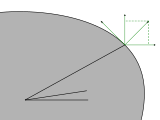
\includegraphics{img/model_development/node_shift_global}
    \caption{Geometric Conditions for Global Node Displacement}
    \label{fig:model_development/node_shift_global}
\end{figure}

In contrast to free surfaces, where the geometric evolution of a node is not constrained by the surrounding space, in grain boundaries the node shifting acts counter the solid material of the other particle.
This introduces additional constraints, since the grain boundary must not form voids and must not overlap.
The geometric constraints are dependent on the local evolution of the grain boundary nodes, as well as the relative position change of the particles.

Starting from a compact grain boundary, meaning that there are no holes and/or overlap present within it, the condition of maintaining the compactness of the grain boundary can be formulated as follows, if the postions of the particles are fixed.
\begin{subequations}
    \begin{align}
        \Step\Shift_{\Normal}\Regarding1 = \Step\Shift_{\Normal}\Regarding2 \\
        \Step\Shift_{\Tangential}\Regarding1 = \Step\Shift_{\Tangential}\Regarding2
    \end{align}
    \label{eq:maintain-compact-particles-fixed}
\end{subequations}

But in reality the positions of particles to each other change, which can be observed macroscopically as shrinkage.
So we formulate instead the total displacement of a node in absolute cartesian space, which must be equal regarded from both particles.
The total node displacement includes contributions from particle displacement (index $\Particle$), normal node displacement (index $\Normal$) and tangential node displacement (index $\Tangential$).
\begin{subequations}
    \begin{align}
        \Step\X_{\Particle1} + \Step\X_{\Normal}^{\Regarding1} + \Step\X_{\Tangential}^{\Regarding1} + \Step\X_{\RotationAngle}^{\Regarding1}
        &= \Step\X_{\Particle2} + \Step\X_{\Normal}^{\Regarding2} + \Step\X_{\Tangential}^{\Regarding2} + \Step\X_{\RotationAngle}^{\Regarding2}\\
        \Step\Y_{\Particle1} + \Step\Y_{\Normal}^{\Regarding1} + \Step\Y_{\Tangential}^{\Regarding1} + \Step\Y_{\RotationAngle}^{\Regarding1}
        &= \Step\Y_{\Particle2} + \Step\Y_{\Normal}^{\Regarding2} + \Step\Y_{\Tangential}^{\Regarding2} + \Step\Y_{\RotationAngle}^{\Regarding2}
        \label{eq:absolute-displacement-contact-constraints}
    \end{align}
\end{subequations}

As can be seen from \cref{fig:model_development/node_shift_global}, the angles of projection of the normal and tangential node shifting to the global cartesian axes are as follows:
\begin{subequations}
    \begin{align}
        \eta_{\Normal} &= \RotationAngle + \Angle + \left( \SurfaceRadiusAngle_{\Lower} + \SurfaceVectorAngle_{\Normal\Lower} - \PI \right)
        \label{eq:global-shift-normal-angle} \\
        \eta_{\Tangential} &= \left( \PI - \SurfaceRadiusAngle_{\Lower} + \SurfaceVectorAngle_{\Tangential\Lower} \right) - \RotationAngle - \Angle
        \label{eq:global-shift-tangential-angle}
    \end{align}
\end{subequations}

With these and further identities on the trigonometric functions the displacements of the node are given as follows:
\begin{subequations}
    \begin{align}
        \Step\X_{\Normal} &= -\Step\Shift_{\Normal} \cos \left( \RotationAngle + \Angle + \SurfaceRadiusAngle + \SurfaceVectorAngle \right)
        \label{eq:global-shift-normal-x} \\
        \Step\Y_{\Normal} &= -\Step\Shift_{\Normal} \sin \left( \RotationAngle + \Angle + \SurfaceRadiusAngle + \SurfaceVectorAngle \right)
        \label{eq:global-shift-normal-y} \\
        \Step\X_{\Tangential} &= \Step\Shift_{\Tangential} \cos \left( \RotationAngle + \Angle + \SurfaceRadiusAngle + \SurfaceVectorAngle \right)
        \label{eq:global-shift-tangential-x} \\
        \Step\Y_{\Tangential} &= \Step\Shift_{\Tangential} \sin \left( \RotationAngle + \Angle + \SurfaceRadiusAngle + \SurfaceVectorAngle \right)
        \label{eq:global-shift-tangential-y}
    \end{align}
\end{subequations}

Inserted in \cref{eq:absolute-displacement-contact-constraints} this leads to two additional constraints for each contact node (grain boundary or neck node), which define the particle displacements $\Step\X_{\Particle i}$ and $\Step\Y_{\Particle i}$ of each particle except one.
Given one grain boundary node (only normal displacement allowed) and two neck nodes per contact, the equation system is unambiguously defined as we have 6 additional constraints (2 per node) for 2 particle displacements and 4 tangential neck node displacements.
Introducing more grain boundary nodes creates more constraints but no additional unknowns (as their normal displacement and flux are covered by the volume balance respectively the optimization).
This leads to an overdetermined system which forces the solution to zero shrinkage (contact nodes are not able to be displaced at all).
Also allowing the grain boundary nodes to be displaced tangentially, leads to an underdetermined system as the contact conditions are not able to determine the particle position anymore.
A solution to this issue has not been found at the time writing this work, so the following applications will be restricted to two neck nodes and one grain boundary node per particle per contact.
This also forbids multiple contacts between the same particles, which is impossible for circular particle geometries but may be for arbitrarily shaped ones.

